%% The first command in your LaTeX source must be the \documentclass command.
%% Options: hf: enable header and footer.
\documentclass[
% twocolumn,
% hf,
]{ceurart}

%% One can fix some overfulls
%\sloppy


%% Minted listings support
%% Need pygment <http://pygments.org/> <http://pypi.python.org/pypi/Pygments>
%\usepackage{minted}
%% auto break lines
%\setminted{breaklines=true}

\usepackage{tikz}
\usepackage{float}
\restylefloat{figure}
\usetikzlibrary{positioning, fit, calc, shapes.geometric, arrows.meta, shadows, backgrounds}
\usepackage{fontawesome5}
%\usepackage{standalone}

\definecolor{paperblue}{RGB}{218, 232, 252}
\definecolor{papergreen}{RGB}{213, 232, 212}
\definecolor{papergray}{RGB}{245, 245, 245}
\definecolor{paperborder}{RGB}{108, 142, 191}
\definecolor{frozengray}{RGB}{102, 102, 102}
\definecolor{bgGray}{RGB}{250, 250, 250}

%%
%% end of the preamble, start of the body of the document source.
\begin{document}

%%
%% Rights management information.
%% CC-BY is default license.
\copyrightyear{2025} % Actualizado para REST-MEX 2025
\copyrightclause{Copyright for this paper by its authors.
  Use permitted under Creative Commons License Attribution 4.0
  International (CC BY 4.0).}

%%
%% This command is for the conference information
\conference{}


%%
%% The "title" command
\title{Modelos Multimodales para Visual Question Answering en Imágenes Histopatológicas}
% \subtitle{Clasificación de Polaridad, Tipo de Destino e Identificación de Pueblos Mágicos} % Subtítulo opcional

% \tnotemark[1] % Si necesitas una nota para el título
% \tnotetext[1]{Este trabajo fue parcialmente financiado por XYZ.}

%%
%% The "author" command and its associated commands are used to define
%% the authors and their affiliations.

% --- Equipo ---
\author[1]{Uziel Lujan Lopez}[
orcid=0009-0001-3160-5294,
email=uziel.lujan@cimat.mx,
]\fnmark[1]

\author[1]{Diego Paniagua-Molina}[
orcid=0009-0006-6564-2794,
email=diego.paniagua@cimat.mx,
]\fnmark[1]


% --- Afiliaciones ---
\address[1]{Mathematics Research Center (CIMAT—Centro de Investigación en Matemáticas), Graduate Program in Statistical Computing, Nuevo León, Mexico}



%% Footnotes
%\cortext[1]{Corresponding author.}
\fntext[1]{Estos autores contribuyeron de igual manera.}


%% Maximo 250 palabras, donde se describa el problema abordado, la base de datos empleada, los métodos utilizados, los resultados obtenidos y las conclusiones principales.
\begin{abstract}
El Visual Question Answering (VQA) en histopatología desafía a la IA a interpretar patrones tisulares complejos y razonar en lenguaje natural, usualmente demandando recursos computacionales prohibitivos. Este trabajo aborda dicho problema bajo restricciones estrictas de hardware, utilizando el dataset PathVQA (32,632 pares QA). Se desarrolló una arquitectura multimodal eficiente integrando CLIP-ViT-Large como encoder visual y TinyLlama-1.1B como modelo de lenguaje, conectados por un proyector MLP y entrenados mediante Full Fine-Tuning en una GPU de 24GB. Esta configuración superó limitaciones de memoria que inviabilizaron modelos más grandes como LLaMA-3. Los resultados demuestran una alta eficacia, alcanzando una exactitud del 86.18\% en preguntas binarias y un 57.76\% de exactitud por palabras clave en preguntas abiertas, validando la capacidad del modelo para identificar conceptos médicos relevantes. Se concluye que es posible construir sistemas de asistencia diagnóstica robustos y accesibles utilizando modelos compactos optimizados, sin depender de infraestructura de hiperescala.
\end{abstract}

%%
%% Entre 3 y 5.
\begin{keywords}
Visual Question Answering, PathVQA, TinyLlama, CLIP, Full Fine-Tuning, Histopathology
\end{keywords}

\maketitle

%--------------------------------------------------------------------------
%	CUERPO DEL ARTÍCULO
%--------------------------------------------------------------------------

% Incluir al menos una pregunta de investigación y formular los objetivos del proyecto bajo la metodologı́a SMART (especı́ficos, medibles, alcanzables, relevantes y con lı́mite de tiempo).
\section{Introducción}

El análisis automatizado de imágenes médicas ha experimentado una revolución con la llegada del aprendizaje profundo. En particular, la tarea de Visual Question Answering (VQA) en el dominio de la histopatología presenta un desafío único: requiere no solo el reconocimiento de patrones visuales complejos en tejidos, sino también la capacidad de razonar sobre ellos y comunicar hallazgos en lenguaje natural.

Si bien existen enfoques previos que combinan encoders visuales como CLIP con decoders de texto simples, estos modelos a menudo carecen de la capacidad de razonamiento profundo. Inicialmente, este proyecto propuso abordar estas limitaciones mediante una arquitectura de vanguardia basada en \textbf{LLaMA-3 (8B)} y el encoder visual \textbf{SigLIP}, ajustados mediante \textbf{LoRA}. Sin embargo, durante la fase experimental, esta configuración enfrentó barreras críticas de infraestructura en el clúster de supercómputo Lab-SB del CIMAT.

El entorno disponible consistía en un nodo de cómputo equipado con tarjetas NVIDIA Titan (24GB VRAM), sin acceso a internet en los nodos de ejecución. A pesar de aplicar técnicas de cuantización de 4-bits, el modelo LLaMA-3 excedía la memoria disponible al cargar los gradientes y estados del optimizador, resultando en errores persistentes de \textit{CUDA Out of Memory (OOM)}. Adicionalmente, se presentaron incompatibilidades técnicas en la integración de SigLIP con la arquitectura LLaVA, lo que impedía un entrenamiento efectivo.

Como respuesta a estos desafíos, el proyecto evolucionó hacia una solución optimizada y robusta: la implementación de una arquitectura basada en \textbf{TinyLlama-1.1B} como modelo de lenguaje y \textbf{CLIP-ViT-Large} como encoder visual. Esta configuración, entrenada mediante \textbf{Full Fine-Tuning (FFT)}, permite equilibrar la capacidad de razonamiento con la eficiencia computacional, garantizando la estabilidad del entrenamiento dentro de los 24GB de VRAM disponibles.

\subsection{Pregunta de Investigación}
Este trabajo busca responder la siguiente interrogante:
\textit{¿Es posible construir un sistema VQA multimodal eficiente y clínicamente coherente para histopatología utilizando modelos compactos (TinyLlama-1.1B) y encoders visuales estándar (CLIP), superando las limitaciones de infraestructura que restringen el uso de LLMs masivos?}

\subsection{Objetivos del Proyecto (SMART)}
El objetivo general es desarrollar y evaluar un sistema VQA para imágenes histopatológicas adaptado a recursos limitados. Desglosado bajo la metodología SMART:

\begin{itemize}
    \item \textbf{Específico (S):} Implementar una arquitectura VQA multimodal integrando TinyLlama-1.1B y CLIP-ViT-Large, utilizando una estrategia de Full Fine-Tuning para asegurar la convergencia y estabilidad del modelo.
    \item \textbf{Medible (M):} Evaluar el desempeño del modelo utilizando el dataset PathVQA, midiendo Accuracy y F1-score para preguntas cerradas (Sí/No), y métricas de generación de texto (BLEU, CIDEr) para preguntas abiertas.
    \item \textbf{Alcanzable (A):} Superar las restricciones de hardware (VRAM) mediante la selección de componentes eficientes y técnicas de optimización (gradient accumulation), logrando un entrenamiento exitoso donde arquitecturas más grandes (LLaMA-3) fallaron.
    \item \textbf{Relevante (R):} Validar la viabilidad de modelos de lenguaje compactos en la patología digital, demostrando que es posible obtener resultados útiles sin requerir infraestructura de hiperescala.
    \item \textbf{Con límite de tiempo (T):} Completar la implementación del pipeline optimizado, el entrenamiento del modelo y la generación del reporte de evaluación antes del 5 de diciembre de 2025.
\end{itemize}


\section{Gestión y Planeación del Proyecto}

Para asegurar la entrega exitosa del proyecto dentro del plazo establecido, se definieron roles claros y se estructuraron las actividades utilizando herramientas de gestión de proyectos, adaptándose a los desafíos técnicos encontrados.

% Roles y responsabilidades
\subsection{Matriz RACI}
Se asignaron responsabilidades específicas a los integrantes del equipo, Uziel Luján (U) y Diego Paniagua (D), para optimizar la colaboración. Uziel se enfocó en la ingeniería del modelo y el entrenamiento en el clúster, mientras que Diego lideró el análisis de métricas y la documentación. La matriz de asignación de responsabilidades (RACI) se detalla en la Tabla \ref{tab:raci}.

\begin{table}[h]
\centering
\caption{Matriz RACI del Proyecto (R: Responsable, A: Aprobador, C: Consultado, I: Informado)}
\label{tab:raci}
\begin{tabular}{|l|c|c|}
\hline
\textbf{Actividad} & \textbf{Uziel (U)} & \textbf{Diego (D)} \\ \hline
Diseño de Arquitectura (TinyLlama + CLIP) & R/A & C \\ \hline
Configuración de Entorno en Clúster & R & I \\ \hline
Preprocesamiento de Datos (PathVQA) & C & R \\ \hline
Entrenamiento del Modelo (FFT) & R & I \\ \hline
Evaluación de Métricas (BLEU, Accuracy) & I & R \\ \hline
Redacción del Reporte Técnico & C & R/A \\ \hline
\end{tabular}
\end{table}

% Diagrama de actividades
\subsection{Método PERT}
El diagrama de evaluación y revisión de programas (PERT) se diseñó para identificar las dependencias entre tareas. La secuencia lógica establecida fue:
\begin{enumerate}
    \item \textbf{Investigación:} Revisión del estado del arte y selección de modelos (TinyLlama, CLIP).
    \item \textbf{Implementación:} Desarrollo del pipeline de datos y arquitectura del modelo.
    \item \textbf{Experimentación:} Pruebas de concepto y resolución de problemas de infraestructura (OOM).
    \item \textbf{Entrenamiento:} Ejecución del Full Fine-Tuning en el clúster.
    \item \textbf{Evaluación:} Cálculo de métricas y análisis de resultados.
    \item \textbf{Cierre:} Documentación final.
\end{enumerate}

% WBS
\subsection{Estructura de Desglose del Trabajo (WBS)}
El proyecto se descompuso en los siguientes paquetes de trabajo principales:
\begin{itemize}
    \item \textbf{1. Gestión de Datos:} Descarga de PathVQA, conversión de formatos y creación de dataloaders.
    \item \textbf{2. Ingeniería de Modelos:} Integración de TinyLlama-1.1B con CLIP-Large, adaptación de dimensiones de embeddings y configuración del tokenizador.
    \item \textbf{3. Infraestructura y Entrenamiento:} Configuración de scripts SLURM, gestión de memoria VRAM y ejecución de ciclos de entrenamiento.
    \item \textbf{4. Aseguramiento de Calidad:} Validación de inferencia, cálculo de métricas automáticas (Accuracy, BLEU) y revisión manual de respuestas.
    \item \textbf{5. Documentación:} Elaboración de bitácora técnica y reporte final.
\end{itemize}

% Identificación de la ruta crı́tica dentro del cronograma.
\subsection{Ruta Crítica y Cronograma}
Dada la fecha límite del 5 de diciembre, la \textbf{ruta crítica} del proyecto se identificó en la fase de \textbf{Entrenamiento y Resolución de Problemas de Infraestructura}. Los fallos iniciales con LLaMA-3 y SigLIP representaron un riesgo significativo de retraso. La decisión de pivotar hacia TinyLlama y CLIP fue crucial para desbloquear esta ruta y permitir tiempo suficiente para la fase de evaluación y reporte. Cualquier retraso adicional en la estabilización del entrenamiento habría hecho imposible cumplir con la entrega.

% Explicación de su uso como estrategia estructurada de resolución de problemas e innovación basada en principios inventivos.
\section{Metodología TRIZ}

Para abordar los bloqueos técnicos críticos encontrados durante el desarrollo, se aplicó la Teoría de Resolución de Problemas Inventivos (TRIZ). Específicamente, se identificó una \textbf{Contradicción Técnica} fundamental: la necesidad de aumentar la \textit{capacidad de razonamiento} del modelo (lo que sugería usar LLaMA-3 8B) entraba en conflicto directo con la limitación de \textit{recursos disponibles} (memoria VRAM estática de 24GB).

Para resolver esta contradicción sin comprometer la viabilidad del proyecto, se aplicaron los siguientes Principios Inventivos:

\begin{itemize}
    \item \textbf{Principio 35: Cambio de Parámetros (Parameter Changes).} En lugar de intentar forzar la ejecución de un modelo masivo mediante cuantización extrema (que falló), se optó por cambiar la propiedad física del sistema: la escala. La sustitución de LLaMA-3 (8B) por TinyLlama (1.1B) permitió eliminar el conflicto de memoria, manteniendo una arquitectura funcional capaz de aprender la tarea.

    \item \textbf{Principio 2: Extracción (Taking Out).} Se identificó que el encoder visual SigLIP, aunque moderno, introducía complejidad innecesaria e incompatibilidades de software ("ruido") que impedían la integración. Se aplicó este principio para "extraer" este componente problemático y reemplazarlo por CLIP, un estándar más estable y compatible con la arquitectura LLaVA, eliminando así la fuente de inestabilidad.

    \item \textbf{Principio 10: Acción Preliminar (Preliminary Action).} Dado que el entorno de ejecución (clúster) carecía de conexión a internet, se anticipó el problema de gestión de dependencias. Se realizó la descarga, conversión de pesos (de \texttt{.bin} a \texttt{.safetensors}) y validación de integridad de los modelos en un entorno local \textit{antes} de la transferencia al clúster. Esta acción previa aseguró que, durante el tiempo de cómputo asignado, el sistema tuviera todos los recursos necesarios listos para usar.
\end{itemize}

% Revisión breve de soluciones previas similares.
\section{Marco Teorico y Trabajos Relacionados}

El campo de Visual Question Answering (VQA) en el dominio médico ha evolucionado drásticamente, transitando desde enfoques discriminativos rígidos hacia sistemas generativos flexibles capaces de razonar.

\subsection{VQA en Patología: Los Inicios}
El trabajo seminal de He et al. \cite{he2020pathvqa}, creadores del dataset PathVQA, estableció los primeros \textit{baselines} utilizando arquitecturas modulares clásicas. Estas combinaban redes convolucionales (como VGG o ResNet) para la visión, con redes recurrentes (LSTM) para el texto. Si bien demostraron la viabilidad de la tarea, operaban bajo un paradigma de clasificación sobre un vocabulario fijo, limitando severamente su capacidad de generalización y razonamiento clínico complejo.

% --- NUEVA SECCIÓN AGREGADA ---
\subsection{Fundamentos del Aprendizaje Multimodal}
Un modelo multimodal se define por su capacidad para procesar y relacionar información proveniente de distintas modalidades sensoriales (e.g., píxeles y palabras) en un espacio semántico común. El desafío central en estos sistemas es el problema de la \textbf{Alineación} (\textit{Alignment}): ¿Cómo lograr que la representación matemática de una "célula tumoral" en una imagen sea equivalente a la representación vectorial de la palabra "tumor" en el modelo de lenguaje?

La arquitectura general para resolver esto, utilizada en sistemas modernos, se compone de tres módulos fundamentales:

\begin{itemize}
    \item \textbf{Encoder Visual (El Ojo):} Transforma la imagen de entrada $I \in \mathbb{R}^{H \times W \times 3}$ en una secuencia de \textit{embeddings} visuales abstractos $Z_v$. Modelos como Vision Transformer (ViT) \cite{dosovitskiy2020image} son estándar aquí por su capacidad de dividir la imagen en "parches".

    \item \textbf{Adaptador o Proyector (El Puente):} Es el componente crítico que "traduce" el lenguaje visual al textual. Matemáticamente, es una función $f_\theta$ (a menudo un MLP o Q-Former) que proyecta los rasgos visuales $Z_v$ al espacio de entrada del LLM, tal que los tokens visuales proyectados $H_v = f_\theta(Z_v)$ sean indistinguibles dimensionalmente de los tokens de texto.

    \item \textbf{Backbone de Lenguaje (El Cerebro):} Un LLM pre-entrenado que recibe la secuencia concatenada de tokens visuales y textuales. Gracias al mecanismo de \textit{Self-Attention}, el modelo puede "atender" a regiones específicas de la imagen mientras procesa la pregunta, generando una respuesta coherente $Y$.
\end{itemize}

Esta arquitectura permite que el modelo no solo "vea", sino que razone sobre la imagen utilizando el vasto conocimiento semántico adquirido por el LLM durante su pre-entrenamiento.

% --- FIN NUEVA SECCIÓN ---

\subsection{Modelos de Visión-Lenguaje (VLMs) en la Actualidad}
Construyendo sobre los fundamentos anteriores, la adaptación de modelos fundacionales ha transformado el estado del arte. Arquitecturas paradigmáticas como \textbf{LLaVA} (Large Language and Vision Assistant) \cite{liu2024visual} implementan esta fusión proyectando características de encoders robustos (como CLIP o SigLIP) directamente hacia LLMs potentes (como LLaMA \cite{touvron2023llama} o Vicuna).

En el contexto médico, la tendencia reciente ha sido utilizar adaptadores eficientes (como LoRA \cite{hu2022lora} o QLoRA) para "enseñar" medicina a estos modelos generales. Sin embargo, existe una barrera importante: la mayoría de estos enfoques (e.g., Med-PaLM, LLaVA-Med) dependen de recursos computacionales masivos (múltiples GPUs A100), lo que limita su reproducibilidad en hospitales o laboratorios modestos.

Nuestra propuesta aborda este hueco específico: demostramos que es posible mantener la arquitectura multimodal sofisticada descrita anteriormente, pero optimizada mediante el uso de modelos compactos (\textbf{TinyLlama}) y encoders eficientes, democratizando así el acceso a herramientas de diagnóstico asistido por IA.

% Descripción detallada de la colección utilizada (origen, caracterı́sticas, tamaño, formato, preprocesamiento, etc.).
\section{Base de Datos}

Para el entrenamiento y evaluación del sistema se utilizó el dataset \textbf{PathVQA} \cite{he2020pathvqa}, una colección de referencia en el dominio de VQA médico. Este conjunto de datos se obtuvo a través de la librería \texttt{datasets} de Hugging Face (repositorio \texttt{flaviagiammarino/path-vqa}), la cual proporciona una versión curada y estandarizada del dataset original.

\subsection{Origen y Composición}
PathVQA se construyó a partir de tres fuentes principales de conocimiento patológico: los libros de texto "Textbook of Pathology" y "Basic Pathology", y la biblioteca digital "Pathology Education Informational Resource" (PEIR). El dataset contiene pares de preguntas y respuestas asociadas a imágenes de microscopía histopatológica.

La versión utilizada en este proyecto consta de un total de \textbf{32,795 pares pregunta-respuesta} distribuidos en \textbf{5,004 imágenes}. Sin embargo, tras un proceso de limpieza de duplicados (tripletas imagen-pregunta-respuesta idénticas), el conjunto efectivo se reduce a \textbf{32,632 muestras} sobre 4,289 imágenes únicas.

\subsection{Estructura y División de Datos}
Cada instancia del dataset es una tripleta compuesta por:
\begin{itemize}
    \item \textbf{Imagen:} Archivo de imagen histopatológica (RGB o CMYK).
    \item \textbf{Pregunta:} Texto en inglés formulando una interrogante clínica (e.g., \textit{"where are liver stem cells located?"}).
    \item \textbf{Respuesta:} Texto en inglés con la respuesta correcta (e.g., \textit{"in the canals of hering"}).
\end{itemize}

\begin{figure}[H]
    \centering
    \includegraphics[width=\linewidth]{figures/muestras_eda.jpeg}
    \caption{Ejemplos representativos del dataset PathVQA. Se muestran imágenes histopatológicas junto con sus correspondientes pares de pregunta y respuesta, ilustrando la variabilidad en tipos de tejido y complejidad de las interrogantes.}
    \label{fig:pathvqa_samples}
\end{figure}

\newpage
El dataset incluye dos tipos principales de preguntas:
\begin{enumerate}
    \item \textbf{Preguntas Binarias (Yes/No):} Requieren una respuesta afirmativa o negativa.
    \item \textbf{Preguntas Abiertas (Open-ended):} Requieren respuestas descriptivas sobre ubicación, identificación de estructuras o diagnóstico.
\end{enumerate}

La división de los datos (splits) utilizada respeta la partición oficial propuesta por los autores para garantizar la comparabilidad de resultados:

\begin{table}[h]
\centering
\caption{Distribución de muestras en PathVQA}
\label{tab:dataset_splits}
\begin{tabular}{|l|c|c|}
\hline
\textbf{Split} & \textbf{Pares QA} & \textbf{Imágenes Únicas} \\ \hline
Entrenamiento (Train) & 19,654 & 2,599 \\ \hline
Validación (Val) & 6,259 & 832 \\ \hline
Prueba (Test) & 6,719 & 858 \\ \hline
\textbf{Total} & \textbf{32,632} & \textbf{4,289} \\ \hline
\end{tabular}
\end{table}

\subsection{Preprocesamiento}
Para adaptar este dataset a la arquitectura multimodal propuesta, se aplicaron las siguientes transformaciones:
\begin{itemize}
    \item \textbf{Imágenes:} Redimensionamiento y normalización para cumplir con la entrada esperada por el encoder CLIP-ViT-Large ($336 \times 336$ píxeles).
    \item \textbf{Texto:} Tokenización utilizando el tokenizador de TinyLlama, añadiendo los tokens especiales de inicio y fin de secuencia requeridos por el modelo de lenguaje.
\end{itemize}

% Descripción de la arquitectura, técnicas y herramientas empleadas.
\section{Propuesta de modelo desarrollado}

La arquitectura implementada es un modelo de Visión-Lenguaje (VLM) basado en el paradigma LLaVA (Large Language and Vision Assistant), adaptado para operar bajo restricciones estrictas de hardware. El sistema integra un encoder visual robusto con un modelo de lenguaje compacto, conectados mediante un proyector multimodal entrenable.

\subsection{Arquitectura del Sistema}
El modelo consta de tres componentes principales, ensamblados mediante una estrategia de "inyección quirúrgica" para evitar la duplicidad de parámetros. La Figura \ref{fig:architecture} ilustra el flujo de información a través de estos componentes.

\begin{enumerate}
    \item \textbf{Encoder Visual (Ojos):} Se utilizó \textbf{CLIP-ViT-Large-Patch14-336} \cite{radford2021learning}. Este modelo procesa imágenes de alta resolución ($336 \times 336$) y genera embeddings visuales ricos. Se seleccionó CLIP sobre SigLIP debido a su estabilidad nativa con la arquitectura LLaVA \cite{liu2024visual} y su compatibilidad comprobada.
    \item \textbf{Proyector Multimodal (Conector):} Un Perceptrón Multicapa (MLP) con activación GELU que proyecta los embeddings visuales al espacio latente del modelo de lenguaje. Este componente es crucial para alinear las representaciones visuales con las textuales.
    \item \textbf{Modelo de Lenguaje (Cerebro):} Se implementó \textbf{TinyLlama-1.1B} \cite{zhang2024tinyllama}, un LLM compacto pero potente. Su tamaño reducido (~1.1 billones de parámetros) permitió realizar un ajuste fino completo (Full Fine-Tuning) en una sola GPU de 24GB, evitando la necesidad de cuantización agresiva que degradaría el rendimiento.
\end{enumerate}

\begin{figure}[H]
    \centering
    % Incluimos el diagrama TikZ directamente o como imagen si se prefiere compilar por separado.
    % Aquí insertamos el código TikZ adaptado para que no sea standalone, o usamos \includegraphics si se generó el PDF.
    % Dado que tenemos el código, lo ideal es incluirlo. Para simplificar en el main, usaremos una versión simplificada o \includegraphics.
    % Asumiendo que el usuario quiere ver el diagrama aquí, insertaré una versión compatible.
    \resizebox{\linewidth}{!}{
        \begin{tikzpicture}[
            node distance=0.8cm and 1.8cm,
            font=\sffamily\small,
            % --- ESTILOS ---
            block/.style={
                rectangle,
                draw=black!60,
                fill=white,
                thick,
                rounded corners=4pt,
                minimum height=1.2cm,
                text width=3.2cm,
                align=center,
                drop shadow
            },
            frozen/.style={
                block,
                draw=frozengray,
                fill=papergray,
                dashed,
                text=frozengray
            },
            trainable/.style={
                block,
                draw=paperborder,
                fill=paperblue,
                very thick
            },
            input_node/.style={
                rectangle,
                rounded corners=6pt,
                draw=black!40,
                fill=white,
                thick,
                minimum height=1.0cm,
                text width=2.5cm,
                align=center,
                font=\sffamily\footnotesize
            },
            operator/.style={
                circle,
                draw,
                thick,
                fill=white,
                inner sep=0pt,
                minimum size=0.8cm,
                font=\large\bfseries
            },
            arrow/.style={
                -{Stealth[length=3mm, width=2mm]},
                thick,
                draw=black!70,
                rounded corners=10pt
            }
        ]

            % =========================================================
            % 1. VISUAL STREAM (Fila Superior) Y=3
            % =========================================================

            \node[input_node] (img_in) at (0, 4.5) {
                \textcolor{paperborder}{\Huge\faImage} \\[0.3em]
                \textbf{Imagen}\\
                \scriptsize $336 \times 336$
            };            \node[frozen, right=of img_in] (clip) {
                \textbf{Visual Encoder}\\
                CLIP-ViT-L\\
                \scriptsize Patch14-336\\
                \faLock \ \textit{Frozen}
            };

            \node[trainable, right=of clip, fill=papergreen, draw=green!40!black] (mlp) {
                \textbf{Proyector}\\
                MLP + GELU\\
                \faCogs \ \textit{Trainable}
            };

            % =========================================================
            % 2. TEXT STREAM (Fila Inferior) Y=0
            % =========================================================

            \node[input_node] (text_in) at (0, 0) {
                \textcolor{paperborder}{\Huge\faQuestionCircle} \\[0.3em]
                \textbf{Prompts}\\
                \scriptsize (Preguntas)
            };

            % Tokenizer alineado horizontalmente con el MLP
            \node[trainable, fill=white, draw=black!50, dashed] (tokenizer) at (mlp |- text_in) {
                \textbf{Tokenizer}\\
                \scriptsize Text Embeddings
            };

            \draw[arrow] (text_in) -- (tokenizer);

            % =========================================================
            % 3. REASONING STREAM (Extremo Derecho)
            % =========================================================

            % Concat posicionado estratégicamente
            \node[operator, label={left:\scriptsize Concat}, right=1.5cm of mlp, yshift=-2.25cm] (concat) {$\parallel$};

            % LLM
            \node[trainable, right=0.8cm of concat, minimum height=2.5cm, fill=paperblue, text width=3.5cm] (llm) {
                \textbf{LLM (Cerebro)}\\
                TinyLlama-1.1B\\
                \textit{(Full Fine-Tuning)}\\[0.5em]
                \faCogs \ \textit{Active Learning}
            };

            % Salida
            \node[input_node, right=0.8cm of llm] (output) {
                \textcolor{paperborder}{\Huge\faComments} \\[0.3em]
                \textbf{Respuesta}
            };

            % =========================================================
            % 4. CONEXIONES
            % =========================================================

            % Visual Stream
            \draw[arrow] (img_in) -- (clip);

            % Clip -> MLP (Con fondo gris en texto para no ensuciar la flecha)
            \draw[arrow] (clip) -- node[midway, above, font=\scriptsize, align=center, fill=bgGray, inner sep=2pt] {Embeds\\(576 tokens)} (mlp);

            % MLP -> Concat
            \draw[arrow] (mlp.east) -| (concat.north)
                node[pos=0.25, above, font=\scriptsize\bfseries, fill=bgGray, inner sep=2pt] {Visual Tokens};

            % Tokenizer -> Concat
            \draw[arrow] (tokenizer.east) -| (concat.south)
                node[pos=0.25, below, font=\scriptsize\bfseries, fill=bgGray, inner sep=2pt] {Text Tokens};

            % Reasoning (Flecha limpia, sin texto "Secuencia Combinada")
            \draw[arrow] (concat) -- (llm);

            % Salida
            \draw[arrow] (llm) -- (output);

            % =========================================================
            % 5. FONDOS DE GRUPO (TÍTULOS CENTRADOS ARRIBA/ABAJO)
            % =========================================================

            \begin{scope}[on background layer]
                % Visual (Arriba) - Título centrado arriba
                \coordinate (phantom_vis) at ($(mlp.north)+(0,0.8)$);
                \node[fit=(img_in)(clip)(mlp)(phantom_vis), fill=bgGray, rounded corners=15pt, draw=black!10, inner sep=15pt, label={[anchor=north, inner sep=5pt, font=\bfseries\color{gray!80}]north:Visual Encoding}] (vis_bg) {};

                % Text (Abajo) - Título centrado abajo (Para simetría y limpieza)
                \coordinate (phantom_text) at ($(tokenizer.south)+(0,-0.6)$);
                \node[fit=(text_in)(tokenizer)(phantom_text), fill=bgGray, rounded corners=15pt, draw=black!10, inner sep=15pt, label={[anchor=south, inner sep=5pt, font=\bfseries\color{gray!80}]south:Text Processing}] (text_bg) {};

                % Reasoning (Derecha) - Título centrado arriba
                \coordinate (phantom_brain) at ($(llm.north)+(0,0.8)$);
                \node[fit=(concat)(llm)(output)(phantom_brain), fill=bgGray, rounded corners=15pt, draw=black!10, inner sep=15pt, label={[anchor=north, inner sep=5pt, font=\bfseries\color{gray!80}]north:Reasoning}] (brain_bg) {};
            \end{scope}

            % =========================================================
            % 6. LEYENDA (Centrada abajo)
            % =========================================================

            \node[draw=black!40, rounded corners, fill=white, anchor=north] (legend) at ($(current bounding box.south) + (0, -0.3)$) {
                \scriptsize
                \begin{tabular}{l l}
                     \faLock \ \textbf{Frozen:} Pesos estáticos & \faCogs \ \textbf{Trainable:} Full Fine-Tuning \\
                \end{tabular}
            };

        \end{tikzpicture}
    }
    \caption{Diagrama de la arquitectura multimodal implementada. Se observa el flujo dual (visual y textual) convergiendo en el LLM TinyLlama, donde el encoder visual CLIP permanece congelado mientras el proyector y el LLM se entrenan activamente.}
    \label{fig:architecture}
\end{figure}

\subsection{Estrategia de Entrenamiento}
A diferencia de enfoques que utilizan adaptadores de bajo rango (LoRA), se optó por una estrategia de \textbf{Full Fine-Tuning (FFT)}.
\begin{itemize}
    \item \textbf{Congelamiento Selectivo:} El encoder visual (CLIP) se mantuvo congelado (frozen) para preservar las características visuales pre-entrenadas.
    \item \textbf{Entrenamiento Activo:} Tanto el proyector multimodal como el modelo de lenguaje (TinyLlama) se mantuvieron entrenables, permitiendo que el sistema aprenda a interpretar las características histopatológicas específicas y a generar respuestas coherentes.
    \item \textbf{Optimizador:} Se utilizó \textbf{AdamW} con una tasa de aprendizaje de $2.0 \times 10^{-5}$ y un esquema de calentamiento (warmup ratio) para garantizar la estabilidad numérica.
\end{itemize}

\subsection{Implementación Técnica y Herramientas}
El desarrollo se realizó utilizando \textbf{PyTorch} y la librería \textbf{Transformers} de Hugging Face. Se implementaron soluciones de ingeniería específicas para superar los desafíos del entorno:
\begin{itemize}
    \item \textbf{Corrección de Tokens (577 vs 576):} Se ajustó la estrategia de selección de características visuales (\texttt{vision\_feature\_select\_strategy="default"}) para eliminar el token CLS sobrante de CLIP, alineando perfectamente los tensores con la entrada esperada por LLaVA.
    \item \textbf{Gestión de Memoria:} Se implementó \textit{Gradient Accumulation} (pasos de 4) para simular un tamaño de lote efectivo mayor sin saturar la VRAM.
    \item \textbf{Logging Offline:} Se desarrolló un sistema de callbacks personalizado (\texttt{FileLoggerCallback}) para registrar métricas en formato JSONL, independiente de servicios en la nube como WandB, inaccesibles desde el clúster.
\end{itemize}

\subsection{Métricas de Evaluación}
Para cuantificar el desempeño del modelo, se utilizaron métricas estándar en VQA y generación de texto, adaptadas a la naturaleza del dataset PathVQA. A continuación se definen formalmente:

\begin{itemize}
    \item \textbf{Accuracy Yes/No:} Diseñada para preguntas binarias, compara solo el primer token de la predicción. Sea $y_i^{GT} \in \{\text{yes},\text{no}\}$ y $f_i^{pred}$ la secuencia generada:
    \begin{equation}
        Accuracy_{Yes/No} = \frac{1}{N} \sum_{i=1}^{N} 1( y_i^{GT} = \text{first}(f_i^{pred}) \big)
    \end{equation}

    \item \textbf{Keyword Accuracy:} Evalúa si el concepto principal correcto (órgano, patología) está presente en la respuesta generada. Sea $k_i$ la palabra clave del GT:
    \begin{equation}
        Accuracy_{Keyword} = \frac{1}{N} \sum_{i=1}^{N} 1( k_i \subseteq f_i^{pred} \big)
    \end{equation}

    \item \textbf{Accuracy Flexible:} Métrica híbrida que considera un acierto si existe coincidencia exacta, inclusión completa o coincidencia del primer token.
    Sea la función auxiliar:
    \begin{equation}
        match(y_i^{GT}, f_i^{pred}) =
        \begin{cases}
        1 & y_i^{GT} = f_i^{pred} \\
        1 & y_i^{GT} \subseteq f_i^{pred} \\
        1 & \text{first}(y_i^{GT}) = \text{first}(f_i^{pred}) \\
        0 & \text{otro caso}
        \end{cases}
    \end{equation}
    Entonces:
    \begin{equation}
        Accuracy_{Flexible} = \frac{1}{N} \sum_{i=1}^{N} match(y_i^{GT}, f_i^{pred})
    \end{equation}

    \item \textbf{BLEU-short:} Adaptación del BLEU clásico optimizada para respuestas cortas (máximo 5 tokens).
    \begin{equation}
        BLEU_{short} = BP \cdot \exp\left( \sum_{n=1}^4 w_n \log p_n^{(5)} \right)
    \end{equation}
    donde $p_n^{(5)}$ es la precisión de n-gramas evaluando solo los primeros 5 tokens.

    \item \textbf{BLEU Clásico:} Incluido por completitud para comparación con literatura previa.
    \begin{equation}
        BLEU = BP \cdot \exp\left( \sum_{n=1}^4 w_n \log p_n \right)
    \end{equation}
\end{itemize}

% Incluir métricas, visualizaciones, gráficas y tablas relevantes. Debes proponer un baseline muy sencillo para comparar los resultados.
\section{Resultados}

Se evaluó el desempeño de dos variantes del modelo: \textbf{TinyLlama-CLIP-768} (versión final con regularización) y \textbf{TinyLlama-CLIP-1024} (versión inicial con mayor contexto). En este análisis, el modelo \textbf{TinyLlama-CLIP-1024} actúa como el \textit{baseline} experimental, permitiendo cuantificar las mejoras introducidas en la versión final optimizada (768).

\subsection{Métricas Cuantitativas y Comparación de Modelos}
La Tabla \ref{tab:results} presenta la comparación directa entre los modelos evaluados. El modelo \textbf{TinyLlama-CLIP-768} demostró ser superior consistentemente en todas las métricas críticas respecto al baseline de 1024 tokens.

\begin{table}[h]
\centering
\caption{Comparación de desempeño en el conjunto de validación (PathVQA). El modelo 768 supera al baseline (1024) en estabilidad (Yes/No) y precisión semántica (Keyword).}
\label{tab:results}
\begin{tabular}{|l|c|c|c|c|c|}
\hline
\textbf{Modelo} & \textbf{Acc Y/N} & \textbf{Acc Flex} & \textbf{Key Acc} & \textbf{BLEU-s} & \textbf{BLEU} \\ \hline
TinyLlama-CLIP-1024 (Baseline) & 82.27\% & 32.58\% & 56.93\% & 0.038 & \textbf{0.024} \\ \hline
\textbf{TinyLlama-CLIP-768} & \textbf{86.18\%} & \textbf{32.90\%} & \textbf{57.76\%} & \textbf{0.038} & 0.022 \\ \hline
\end{tabular}
\end{table}

Los resultados indican que la reducción de la ventana de contexto y la aplicación de regularización en el modelo 768 mejoraron significativamente la \textbf{Accuracy Yes/No} (+3.91\%), lo que sugiere una mayor estabilidad en la toma de decisiones binarias críticas para el diagnóstico.

\begin{figure}[H]
    \centering
    \includegraphics[width=\linewidth]{figures/summary_metrics_comparison.png}
    \caption{Comparación visual de métricas entre los modelos TinyLlama-CLIP-768 y TinyLlama-CLIP-1024. Se aprecia la superioridad del modelo 768 en métricas clave.}
    \label{fig:metrics_comparison}
\end{figure}

\subsection{Dinámica de Entrenamiento}
La Figura \ref{fig:training_curves_comparison} muestra la curvas de aprendizaje para ambos modelos VQA. Se observa una convergencia estable.

\begin{figure}[H]
    \centering
    \begin{minipage}{0.48\textwidth}
        \centering
        \includegraphics[width=\linewidth]{figures/training_plot_768.png}
        \caption{TinyLlama-CLIP-768.}
        \label{fig:training_curve}
    \end{minipage}\hfill
    \begin{minipage}{0.48\textwidth}
        \centering
        \includegraphics[width=\linewidth]{figures/training_plot_1024.png}
        \caption{TinyLlama-CLIP-1024.}
        \label{fig:training_curve_1024}
    \end{minipage}
    \caption{Curvas de aprendizaje comparativas. Izquierda: Modelo final (768 tokens) mostrando convergencia estable. Derecha: Baseline (1024 tokens).}
    \label{fig:training_curves_comparison}
\end{figure}

\subsection{Análisis Cualitativo}
La Figura \ref{fig:samples} presenta ejemplos de inferencia del modelo. Se observa que el sistema es capaz de identificar correctamente estructuras histológicas y responder preguntas sobre tinción y morfología.

\begin{figure}[H]
    \centering
    \begin{minipage}{0.48\textwidth}
        \centering
        \includegraphics[width=\linewidth]{figures/sample_validation_02349.png}
        %\caption{Ejemplo 1}
    \end{minipage}\hfill
    \begin{minipage}{0.48\textwidth}
        \centering
        \includegraphics[width=\linewidth]{figures/sample_validation_04163.png}
        %\caption{Ejemplo 2}
    \end{minipage}

    \vspace{0.5cm}

    \begin{minipage}{0.48\textwidth}
        \centering
        \includegraphics[width=\linewidth]{figures/sample_validation_04770.png}
        %\caption{Ejemplo 3}
    \end{minipage}\hfill
    \begin{minipage}{0.48\textwidth}
        \centering
        \includegraphics[width=\linewidth]{figures/sample_validation_05335.png}
        %\caption{Ejemplo 4}
    \end{minipage}

    \vspace{0.5cm}

    \begin{minipage}{0.48\textwidth}
        \centering
        \includegraphics[width=\linewidth]{figures/sample_validation_05786.png}
        %\caption{Ejemplo 5}
    \end{minipage}\hfill
    \begin{minipage}{0.48\textwidth}
        \centering
        \includegraphics[width=\linewidth]{figures/sample_validation_04933.png}
        %\caption{Ejemplo 6}
    \end{minipage}

    \caption{Muestras de predicciones del modelo en el conjunto de validación. El modelo genera respuestas coherentes alineadas con la pregunta visual.}
    \label{fig:samples}
\end{figure}

\subsection{Análisis de Errores}
Un análisis cualitativo detallado de las predicciones incorrectas revela patrones consistentes que explican las limitaciones actuales del modelo:

\begin{itemize}
    \item \textbf{Verborrea y Ruido Semántico:} Ambos modelos, especialmente la versión de 1024 tokens, tienden a generar descripciones excesivamente detalladas. Aunque la información clínica añadida suele ser plausible, introduce "ruido" que penaliza métricas de coincidencia exacta. Por ejemplo, ante la pregunta \textit{"what organ is shown?"}, el modelo puede responder \textit{"liver with metastatic appearance..."} en lugar de simplemente \textit{"liver"}.

    \item \textbf{Alucinación de Detalles (Modelo 1024):} El modelo con mayor contexto (1024) mostró una mayor propensión a inventar condiciones patológicas no presentes en la imagen (e.g., mencionar "inflamación" o "quistes" sin evidencia clara), lo que justifica la elección del modelo 768 como la versión final más robusta.

    \item \textbf{Generalización vs. Especificidad:} El sistema demuestra una alta capacidad para identificar la región anatómica general (e.g., "kidney region"), pero ocasionalmente falla al distinguir subestructuras específicas (e.g., "renal cortex"), lo cual es esperable dado que el encoder visual se mantuvo congelado y no se especializó en texturas finas de histopatología.
\end{itemize}

% Análisis crı́tico de los resultados, limitaciones del enfoque y posibles lı́neas de mejora.
\section{Discusión}

Los resultados obtenidos validan la hipótesis de que es posible construir sistemas VQA competentes para el dominio médico utilizando arquitecturas compactas, siempre que se apliquen estrategias de entrenamiento adecuadas como el Full Fine-Tuning.

\subsection{Análisis de Desempeño}
El alto rendimiento en preguntas binarias (86.18\%) sugiere que el encoder CLIP-ViT-Large es eficaz para extraer características discriminativas en imágenes histopatológicas, incluso sin un ajuste fino de sus pesos (frozen). Esto confirma la robustez de las representaciones visuales pre-entrenadas de CLIP.

Por otro lado, la brecha significativa entre la \textit{Accuracy General} (32.80\%) y la \textit{Keyword Accuracy} (57.76\%) resalta una limitación intrínseca de las métricas basadas en coincidencia exacta. El modelo frecuentemente genera la respuesta correcta semánticamente (e.g., "tumor cells") pero es penalizado por no coincidir palabra por palabra con la referencia (e.g., "tumor"). Esto indica que el modelo ha aprendido los conceptos médicos, pero requiere un refinamiento en la generación de lenguaje para alinearse con el estilo conciso del dataset.

\subsection{Limitaciones Técnicas}
A pesar del éxito en la implementación, el enfoque presenta limitaciones claras:
\begin{itemize}
    \item \textbf{Resolución Visual:} La entrada de $336 \times 336$ píxeles, impuesta por la arquitectura de CLIP, puede ser insuficiente para detectar patologías que dependen de detalles celulares finos o texturas sutiles a gran aumento.
    \item \textbf{Capacidad del LLM:} Aunque TinyLlama es eficiente, su capacidad de razonamiento complejo es inferior a modelos de 7B+ parámetros. Esto se refleja en el bajo puntaje BLEU (0.022), sugiriendo dificultades para construir oraciones largas y gramaticalmente complejas que coincidan con las referencias.
    \item \textbf{Sesgo del Dataset:} PathVQA tiene un desbalance hacia preguntas de tipo "Sí/No". Si bien el modelo maneja bien este tipo, su capacidad generativa en preguntas abiertas ("Open-ended") aún tiene margen de mejora.
\end{itemize}

\subsection{Líneas de Mejora Futura}
Para superar estas barreras en iteraciones futuras, se proponen las siguientes estrategias:
\begin{enumerate}
    \item \textbf{Encoders de Mayor Resolución:} Explorar variantes de CLIP o SigLIP que soporten resoluciones mayores (e.g., $448^2$ o estrategias de \textit{tiling}) para capturar mejor la morfología celular.
    \item \textbf{Métricas Semánticas:} Incorporar métricas de evaluación basadas en embeddings (como BERTScore) o evaluación asistida por LLMs (LLM-as-a-judge) para valorar la corrección semántica de las respuestas más allá de la coincidencia exacta.
    \item \textbf{Data Augmentation:} Implementar técnicas de aumento de datos específicas para VQA (e.g., reformulación de preguntas, rotación de imágenes) para mejorar la robustez y generalización del modelo.
\end{enumerate}

% Sı́ntesis final de hallazgos y aportaciones.
\section{Conclusiones}

Este proyecto ha demostrado la viabilidad técnica y práctica de desarrollar sistemas de Visual Question Answering para el dominio histopatológico en entornos de cómputo restringidos. La principal aportación de este trabajo reside en la validación de una arquitectura eficiente que combina un modelo de lenguaje compacto (\textbf{TinyLlama-1.1B}) con un encoder visual robusto (\textbf{CLIP-ViT-Large}), logrando un equilibrio óptimo entre rendimiento y consumo de recursos.

Los hallazgos experimentales indican que no es estrictamente necesario recurrir a modelos masivos (como LLaMA-3 8B o GPT-4) para obtener resultados competentes en tareas especializadas. Con una exactitud del \textbf{86.18\%} en preguntas binarias y una capacidad notable para recuperar conceptos clave en preguntas abiertas (\textbf{57.76\%}), el modelo propuesto se perfila como una herramienta de asistencia preliminar útil para la educación y el triaje en patología digital.

Finalmente, la superación de los desafíos de infraestructura mediante la aplicación de principios de ingeniería (Gradient Accumulation, gestión de memoria) y metodología TRIZ subraya la importancia de la optimización de software sobre la fuerza bruta del hardware. Este enfoque democratiza el acceso a la inteligencia artificial médica, permitiendo que laboratorios con recursos limitados puedan investigar y desplegar soluciones de vanguardia.

\section{Disponibilidad de Recursos}
El código fuente completo, los scripts de entrenamiento y la documentación detallada del proyecto se encuentran disponibles públicamente en el siguiente repositorio de GitHub: \url{https://github.com/UzielLujan/multimodal-vqa-project}.

% Bajo un formato académico uniforme (APA o IEEE).
\bibliography{refs.bib}

%%
%% If your work has an appendix, this is the place to put it.
% \appendix
% \section{Título del Apéndice A}
% ...

\end{document}
%%
%% End of file
